\documentclass[border=5pt]{standalone}
\usepackage{tikz}
\usepackage{xcolor}
\usetikzlibrary{positioning}

\begin{document}
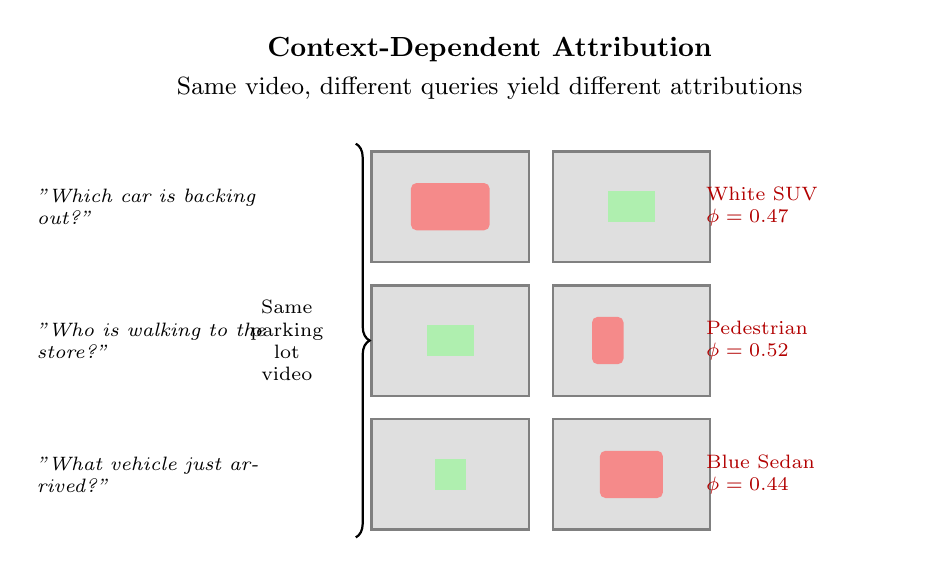
\begin{tikzpicture}[
    frame/.style={draw=gray, thick, minimum width=2cm, minimum height=1.4cm, fill=gray!25},
    query/.style={font=\scriptsize\itshape, text width=3.5cm, align=left},
    result/.style={font=\scriptsize, text width=2.5cm, align=left},
]

% Title
\node[font=\bfseries] at (4, 5.5) {Context-Dependent Attribution};
\node[font=\small] at (4, 5) {Same video, different queries yield different attributions};

% Row 1
\node[query] at (0, 3.5) {"Which car is backing out?"};
\node[frame] (f1a) at (3.5, 3.5) {};
\node[frame] (f1b) at (5.8, 3.5) {};
\fill[red!60, opacity=0.7, rounded corners=2pt] (3.0, 3.2) rectangle (4.0, 3.8);
\node[result, red!70!black] at (8, 3.5) {White SUV\\$\phi = 0.47$};

% Row 2
\node[query] at (0, 1.8) {"Who is walking to the store?"};
\node[frame] (f2a) at (3.5, 1.8) {};
\node[frame] (f2b) at (5.8, 1.8) {};
\fill[red!60, opacity=0.7, rounded corners=2pt] (5.3, 1.5) rectangle (5.7, 2.1);
\node[result, red!70!black] at (8, 1.8) {Pedestrian\\$\phi = 0.52$};

% Row 3
\node[query] at (0, 0.1) {"What vehicle just arrived?"};
\node[frame] (f3a) at (3.5, 0.1) {};
\node[frame] (f3b) at (5.8, 0.1) {};
\fill[red!60, opacity=0.7, rounded corners=2pt] (5.4, -0.2) rectangle (6.2, 0.4);
\node[result, red!70!black] at (8, 0.1) {Blue Sedan\\$\phi = 0.44$};

% Brackets showing same video
\draw[thick, decorate, decoration={brace, amplitude=5pt}]
    (2.3, 4.3) -- (2.3, -0.7) node[midway, left=8pt, font=\scriptsize, align=center] {Same\\parking\\lot\\video};

% Green boxes for non-important objects in each row
\fill[green!50, opacity=0.5] (5.5, 3.3) rectangle (6.1, 3.7);
\fill[green!50, opacity=0.5] (3.2, 1.6) rectangle (3.8, 2.0);
\fill[green!50, opacity=0.5] (3.3, -0.1) rectangle (3.7, 0.3);

\end{tikzpicture}
\end{document}
